%!TEX TS-program=xelatex
%!USE flag=shell-escape
\documentclass{beamer}
\usepackage{HSE-theme/beamerthemeHSE} % Подгружаем тему

%%% Работа с русским языком и шрифтами
\usepackage[english,russian]{babel}   % загружает пакет многоязыковой вёрстки
\usepackage{fontspec}      % подготавливает загрузку шрифтов Open Type, True Type и др.
\defaultfontfeatures{Ligatures={TeX},Renderer=Basic}  % свойства шрифтов по умолчанию
\setmainfont[Ligatures={TeX,Historic}]{Myriad Pro} %  установите шрифты Myriad Pro или (при невозможности) замените здесь на другой шрифт, который есть в системе — например, Arial
\setsansfont{Myriad Pro}  %  установите шрифты Myriad Pro или (при невозможности) замените здесь на другой шрифт, который есть в системе — например, Arial
\setmonofont{Courier New}
\uselanguage{russian}
\languagepath{russian}
\deftranslation[to=russian]{Theorem}{Теорема}
\deftranslation[to=russian]{Definition}{Определение}
\deftranslation[to=russian]{Definitions}{Определения}
\deftranslation[to=russian]{Corollary}{Следствие}
\deftranslation[to=russian]{Fact}{Факт}
\deftranslation[to=russian]{Example}{Пример}
\deftranslation[to=russian]{Examples}{Примеры}

\usepackage{multicol}       % Несколько колонок
\graphicspath{{images/}}    % Папка с картинками

% графики всякие
\usepackage{qtree}
\usepackage{pgfplots}
    \pgfplotsset{
        compat=1.12,
    }

% \usepackage[backend=biber]{biblatex}
% \addbibresource{used_sources.bib}
\usepackage{caption}
\captionsetup{labelformat=simple}
\newlength{\mylen}


%%% Информация об авторе и выступлении
\title[Заголовок]{\footnotesize Факультет Компьютерных Наук\\Департамент
Программной Инженерии\\Отчёт по преддипломной практике}
\subtitle{Криптографические алгоритмы и протоколы для распределенных реестров\\
Cryptographic Algorithms and Protocols for Distributed Ledgers}
\author[Куприянов К.И.]{\scriptsize Выполнил: студент
гр.БПИ151 Куприянов Кирилл\\Научный руководитель: Профессор, руководитель ДПИ,\\к.т.н. Авдошин Сергей Михайлович}
\institute[Высшая школа экономики]{}
\date{\the\year}

\begin{document}    % Начало презентации
\frame[plain]{
    \maketitle
}

% \frame[plain]{\titlepage} % Титульный слайд

% \section{Просто слайд с текстом}
% \subsection{Просто слайд с текстом}

\begin{frame}
\frametitle{Предметная область}
    \begin{multicols}{2}
        1. Распределённые реестры -- ``база данных'', которая распределена между
        несколькими сетевыми узлами или вычислительными устройствами. Каждый
        узел получает данные из других узлов и хранит полную копию реестра.
        Обновления узлов происходят независимо друг от друга

        \columnbreak

        2. Криптография -- наука, изучающая математические методы защиты
        информации, методы преобразования, обеспечивающие ее конфиденциальность
        и аутентичность.\\
        \emph{Разделы: асимметричные криптосистемы, системы электронной цифровой
        подписи (ЭЦП), хеш-функции}
        \medskip
        % \includegraphics[width=\columnwidth]{skidka.png}
    \end{multicols}
\end{frame}

\begin{frame}
\frametitle{Определения}
        \begin{itemize}
\small
    \item Распределённый реестр (Distributed Ledger) --- Распределённая база
        данных между сетевыми узлами. Каждый из узлов может получать данные
                других, при этом храня полную копию реестра.  Обновления этих
                узлов происходят независимо друг от друга

    \item Блокчейн --- Постоянно растущий список записей, называемых блоками,
        которые связаны и защищены с помощью криптографии. Он копируется его
                пользователями и устойчив к модификации

    \item DAG --- Направленный ациклический граф. Это ориентированный граф с
        данными, использующий топологическую сортировку (от ранних узлов к
                более поздним)
    \item Протокол консенсуса --- стандарт, описывающий правила взаимодействия
        и способы достижения согласия в группе. Голосование происходит в пользу
                большинства, не учитывая интересы меньшинства, но с другой
                стороны, это гарантирует достижение соглашения, которое несет
                пользу всей группе
        \end{itemize}
\end{frame}

\begin{frame}
\frametitle{Оглавление ВКР}
    \begin{itemize}
\small
        \item Реферат {\bfseries \color{green!75!blue}(95\%)}
        \item Введение {\bfseries \color{green!75!blue}(95\%)}
        \item Глава 1. Обзор распределённых реестров {\bfseries \color{green!75!blue}(95\%)}
        \item Глава 2. Теоретический анализ алгоритмов и протоколов {\bfseries \color{yellow!75!green}(15\%)}
        \item Глава 3. Реализация программной библиотеки {\bfseries \color{red!75!blue}(0\%)}
        \item Заключение {\bfseries \color{green!75!blue}(80\%)}
        \item Приложение А. Техническое задание {\bfseries \color{green!75!blue}(95\%)}
        \item Приложение Б. Руководство оператора  {\bfseries \color{red!75!blue}(0\%)}
        \item Приложение В. Программа и методика испытаний {\bfseries \color{red!75!blue}(0\%)}
        \item Приложение Г. Текст программы {\bfseries \color{red!75!blue}(0\%)}
    \end{itemize}
\end{frame}

\begin{frame}[c]
    \frametitle{Обоснование актуальности работы}
    \begin{itemize}
        \item Популярность темы (TON, IPFS)
        \item Устаревшая существующая классификация (на 2014 г.)
        \item Люди опираются на бизнес аналитику
        \item Отсутствие библиотеки с реализациями алгоритмов
    \end{itemize}
\end{frame}

\begin{frame}[c]
    \frametitle{Обоснование актуальности работы}
    \begin{multicols}{2}
    \begin{figure}
        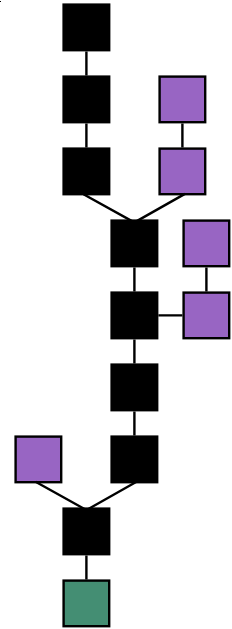
\includegraphics[height=0.8\columnwidth]{blockchain.png}
        \caption{Блокчейн}
    \end{figure}
        \columnbreak
    \begin{figure}
        
\includegraphics[height=0.8\columnwidth]{ton.png}
        \caption{Криптовалюты}
    \end{figure}
\end{multicols}
\end{frame}

\begin{frame}[c]
    \frametitle{Криптопротокол 2014г.}
    \begin{figure}
        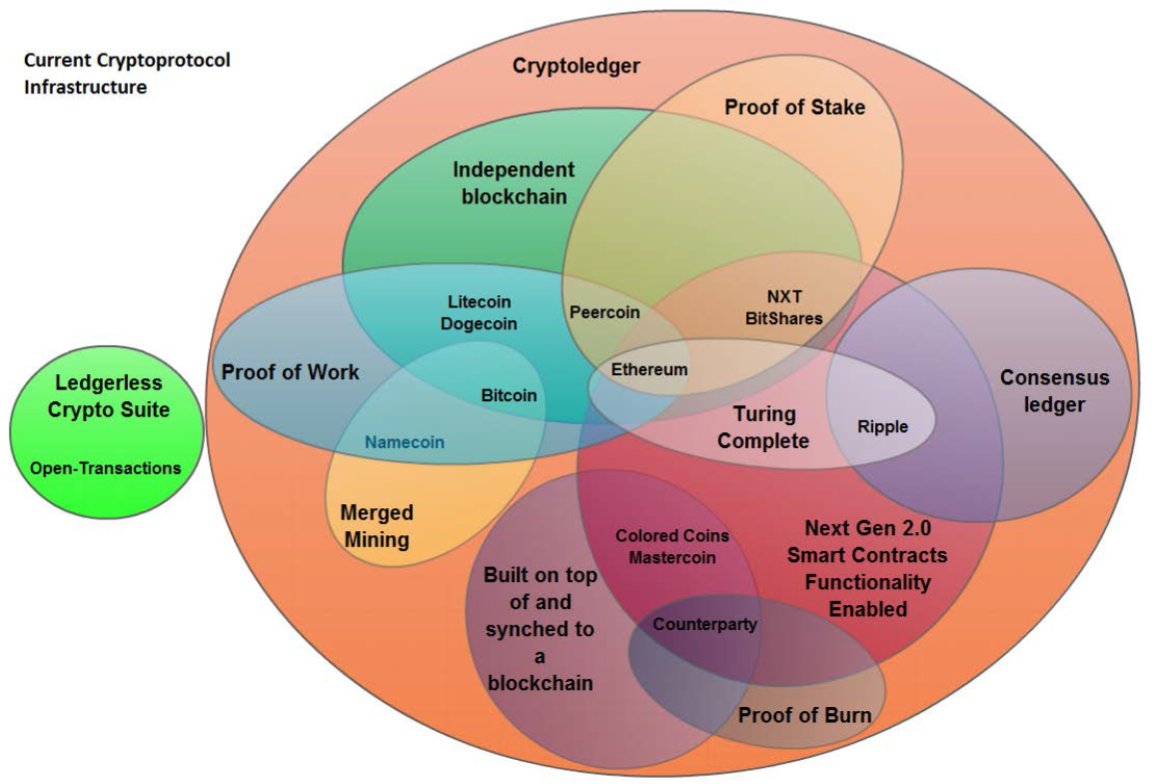
\includegraphics[height=0.5\columnwidth]{current_protocols}
        \caption{Криптопротокол по состоянию на 2014 год [15]}
    \end{figure}
\end{frame}

\begin{frame}
    \frametitle{Цель и задачи работы}
    \textbf{Цель}: Анализ и классификация актуальных криптографических
    алгоритмов для распределённых реестров в мире\\
    \textbf{Задачи}:
    \begin{itemize}
        \item Выявить популярные распределённые реестры; выделить и изучить
              криптографические алгоритмы в них
        \item Изучить особенности реализации алгоритмов
        \item Расположить их на диаграмме Эйлера-Венна для создания новой классификации
        \item Написать библиотеку криптографических алгоритмов и протоколов
    \end{itemize}
\end{frame}

\begin{frame}
    \frametitle{Распределённые реестры}
    \begin{figure}[h]
        \captionsetup{labelformat=parens}
        \Tree [.DL [.DAG ] [.Blockchain ] [.Hybrids\ \&\ Others ]]
        \caption{Виды распределённых реестров}\label{graph_reester}
    \end{figure}
\end{frame}

\begin{frame}
    \frametitle{Классификация по открытости}
    \begin{multicols}{3}
        \textbf{Канада}
        \begin{itemize}
            \item Public
            \item Private
            \item Consortium
        \end{itemize}
        \columnbreak
        \textbf{Великобритания}
         \begin{itemize}
                 \small
             \item Permissioned private
             \item Permissioned public
             \item Unpermissioned public
         \end{itemize}
        \columnbreak
        \textbf{Россия}
        \begin{itemize}
            \item Public
            \item Private
        \end{itemize}
    \end{multicols}
\end{frame}

\begin{frame}
    \frametitle{Алгоритмы и протоколы}
    \begin{multicols}{3}
        \textbf{Протоколы консенсусa}
        \vspace{0.35cm}
        \begin{itemize}
            \item PoW
            \item PoS
            \item DPoS
            \item PoA
            \item PoWeight
            \item BFT
        \end{itemize}
        \columnbreak
        \textbf{Алгоритмы хэширования}
        \vspace{0.56cm}
         \begin{itemize}
             \item SHA-256
             \item SHA-512
             \item Scrypt
             \item KECCAK-256
             \item Ethash
             \item X11
             \item X17
             \item Lyra2rev2
             \item myr-groestl
             \item blake2s
         \end{itemize}
        \columnbreak
        \textbf{Алгоритмы генерации случайных чисел}
        \begin{itemize}
            \item DRBG
            \item CPRNG
        \end{itemize}
    \end{multicols}
\end{frame}

\begin{frame}
    \frametitle{Существующая классификация криптопротоколов}
    \framesubtitle{На 2014 год}
    \textbf{Задача: } Расширение классификации

    \begin{figure}
        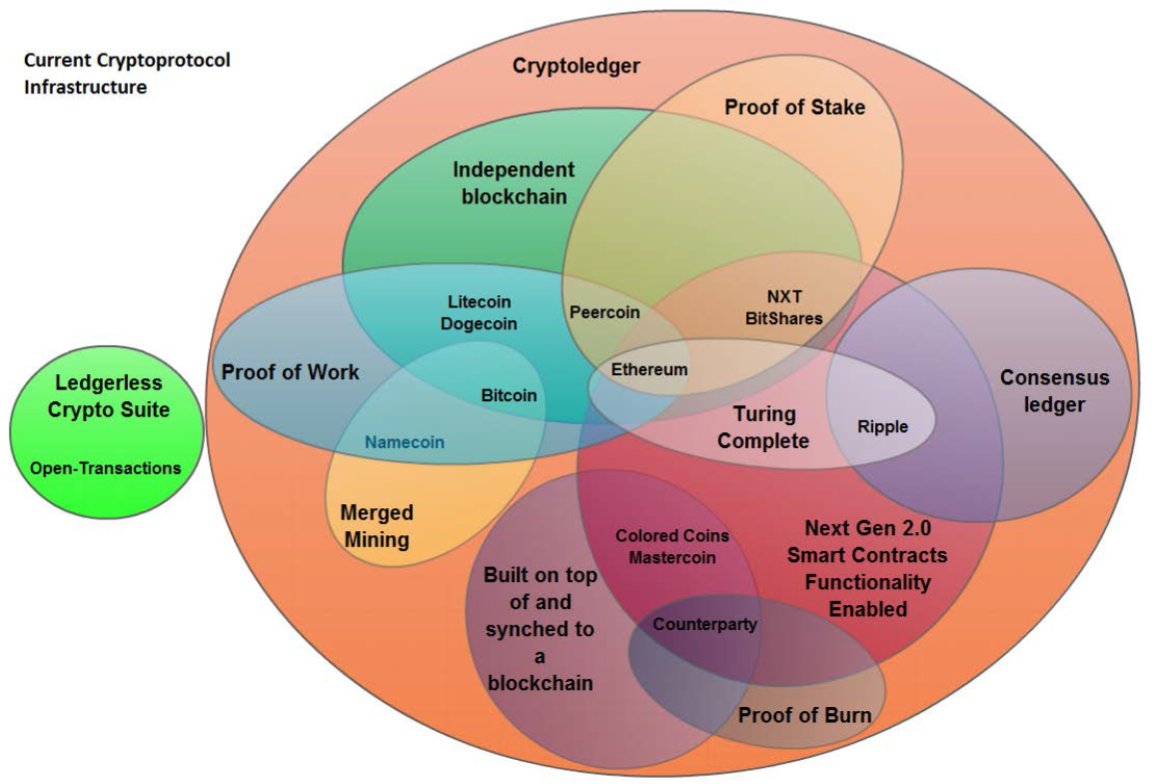
\includegraphics[width=0.75\columnwidth]{current_protocols.png}
        \caption{Криптопротокол по состоянию на 2014 год [15]}
    \end{figure}
\end{frame}

\begin{frame}
    \frametitle{Существующая классификация криптопротоколов*}
    \framesubtitle{На 2019 год}
    \textbf{Результат: } Расширенная классификация

    \begin{figure}
        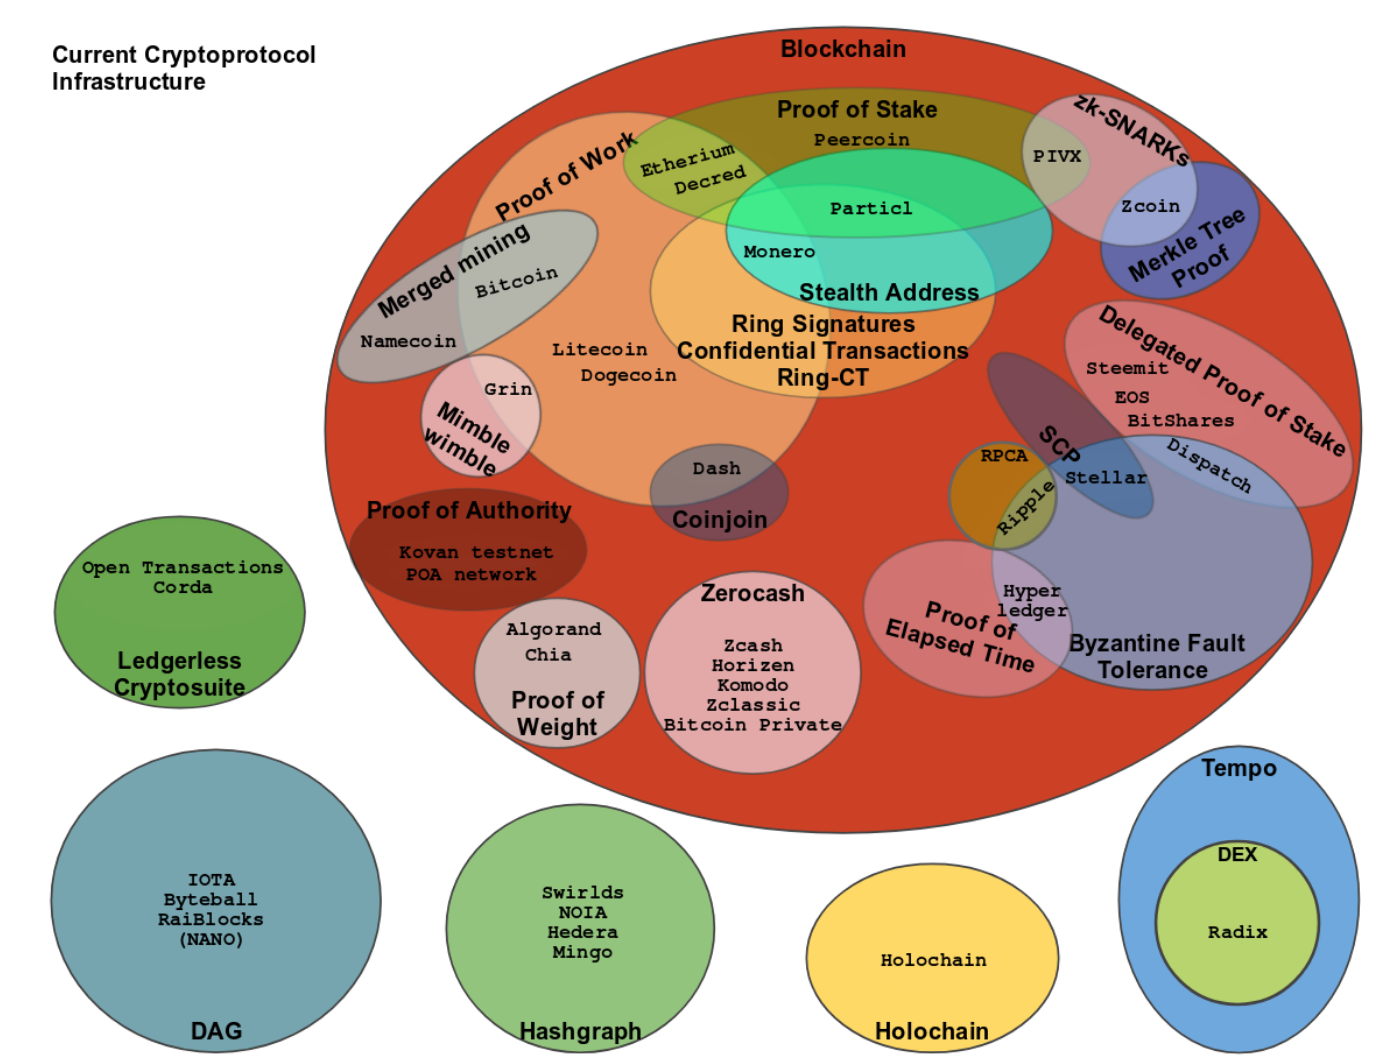
\includegraphics[width=0.65\columnwidth]{myprotocol_w_title.png}
        \caption{Криптопротокол по состоянию на 2019 год*}
    \end{figure}
    \begin{flushright}
        \vspace{-0.5cm}
        \tiny
        *Альфа версия
    \end{flushright}
\end{frame}

\begin{frame}
    \frametitle{Общее}
    \framesubtitle{Сравнительный анализ}
    \begin{figure}
        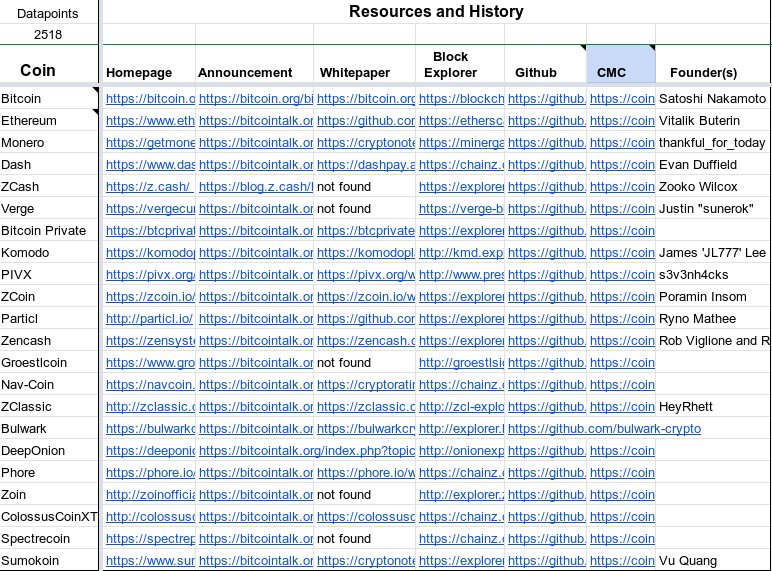
\includegraphics[width=0.79\columnwidth]{sravn1.png}
        \caption{Необходимые ресурсы для анализа}
    \end{figure}
\end{frame}

\begin{frame}
    \frametitle{Алгоритмы}
    \framesubtitle{Сравнительный анализ}
    \begin{figure}
        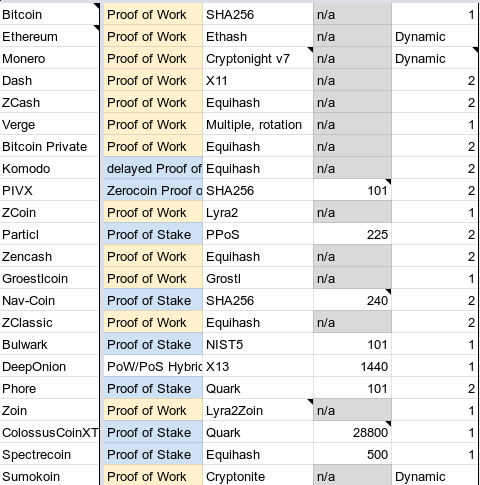
\includegraphics[width=0.6\columnwidth]{sravn2.png}
        \caption{Алгоритмы хэширования, протоколы консенсуса и др.}
    \end{figure}
\end{frame}

\begin{frame}
    \frametitle{Алгоритмы, обеспечивающие приватность}
    \framesubtitle{Сравнительный анализ}
    \begin{figure}
        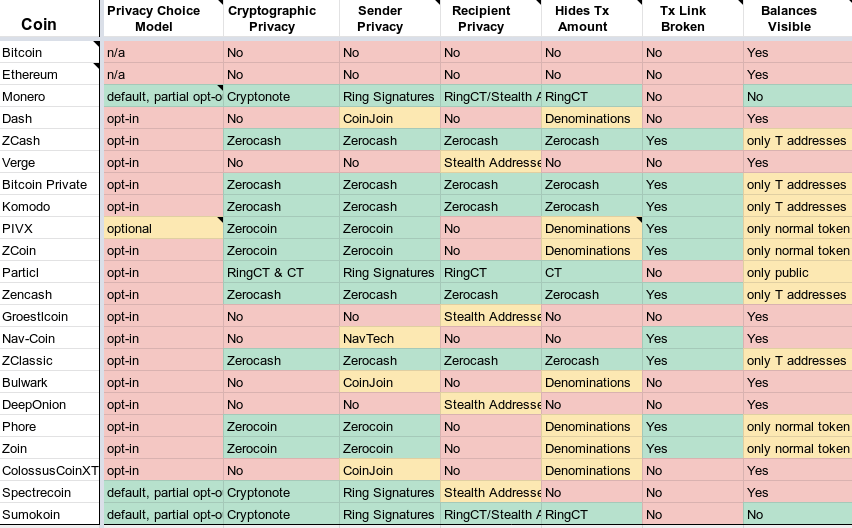
\includegraphics[width=\columnwidth]{sravn3.png}
        \caption{Алгоритмы, обеспечивающие приватность}
    \end{figure}
\end{frame}

\begin{frame}
    \frametitle{Методы, алгоритмы и технологии}
    \begin{multicols}{2}
        \begin{itemize}
            \item Сравнительный анализ алгоритмов и протоколов
            \item Язык Python 3.6.5
            \item {\LaTeX} (дистрибутив XeTeX) для презентаций и текста
            \item YAML 1.2 как язык конфигурации библиотеки
            \item Лицензии на использование и распространение кодов
        \end{itemize}
        \bigskip
        \columnbreak
        \begin{figure}
            
\includegraphics[width=\columnwidth]{tech.png}
        \end{figure}
    \end{multicols}
\end{frame}

\begin{frame}
    % \frametitle{}
    \begin{multicols}{2}
        \begin{center}
            \textbf{Сделано}
        \end{center}
        \begin{itemize}
            \item Исследовательская часть {\bfseries \color{yellow!60!green}(70\%)}
            \item Программа {\bfseries \color{green!75!blue}(80\%)}
            \item Документация {\bfseries \color{red!75!blue}(25\%)}
        \end{itemize}
        \bigskip
        \columnbreak
        \begin{center}
            \textbf{\#TODO}
        \end{center}
        \begin{itemize}
            \item Завершить классификацию
            \item Доработать полный обзор рассмотренных алгоритмов
            \item Проверить лицензии всех предполагаемых используемых кодов
            \item Добавить в программу генерацию кода (Python Metaprogramming)
        \end{itemize}
    \end{multicols}
\end{frame}

\begin{frame}
    \frametitle{Список используемых источников}
    \begin{figure}
        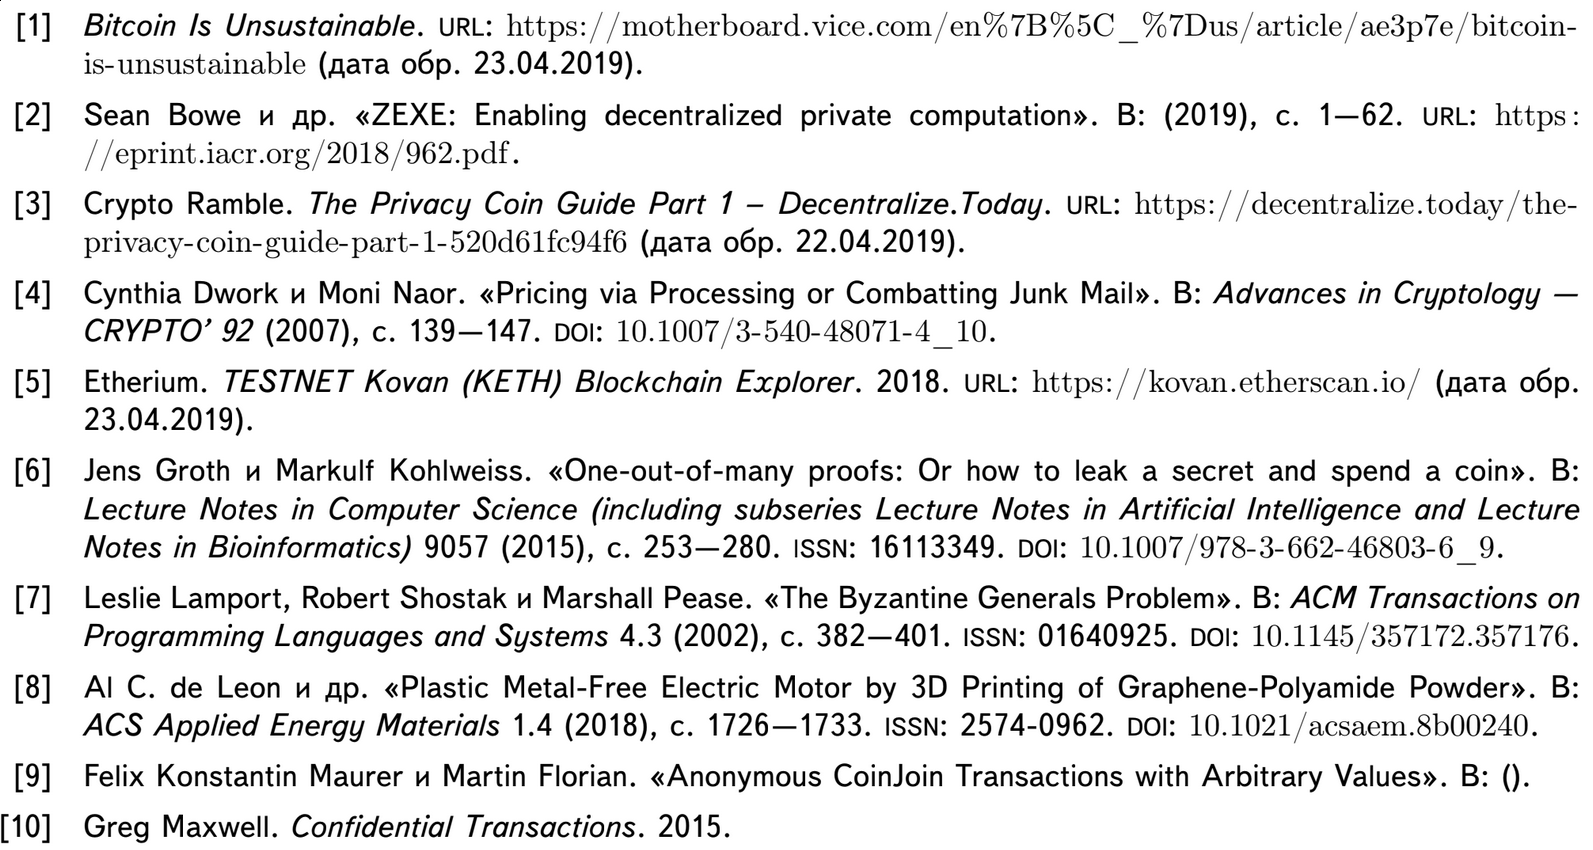
\includegraphics[width=\columnwidth]{lit1.png}
    \end{figure}
\end{frame}

\begin{frame}
    \frametitle{Список используемых источников}
    \begin{figure}
        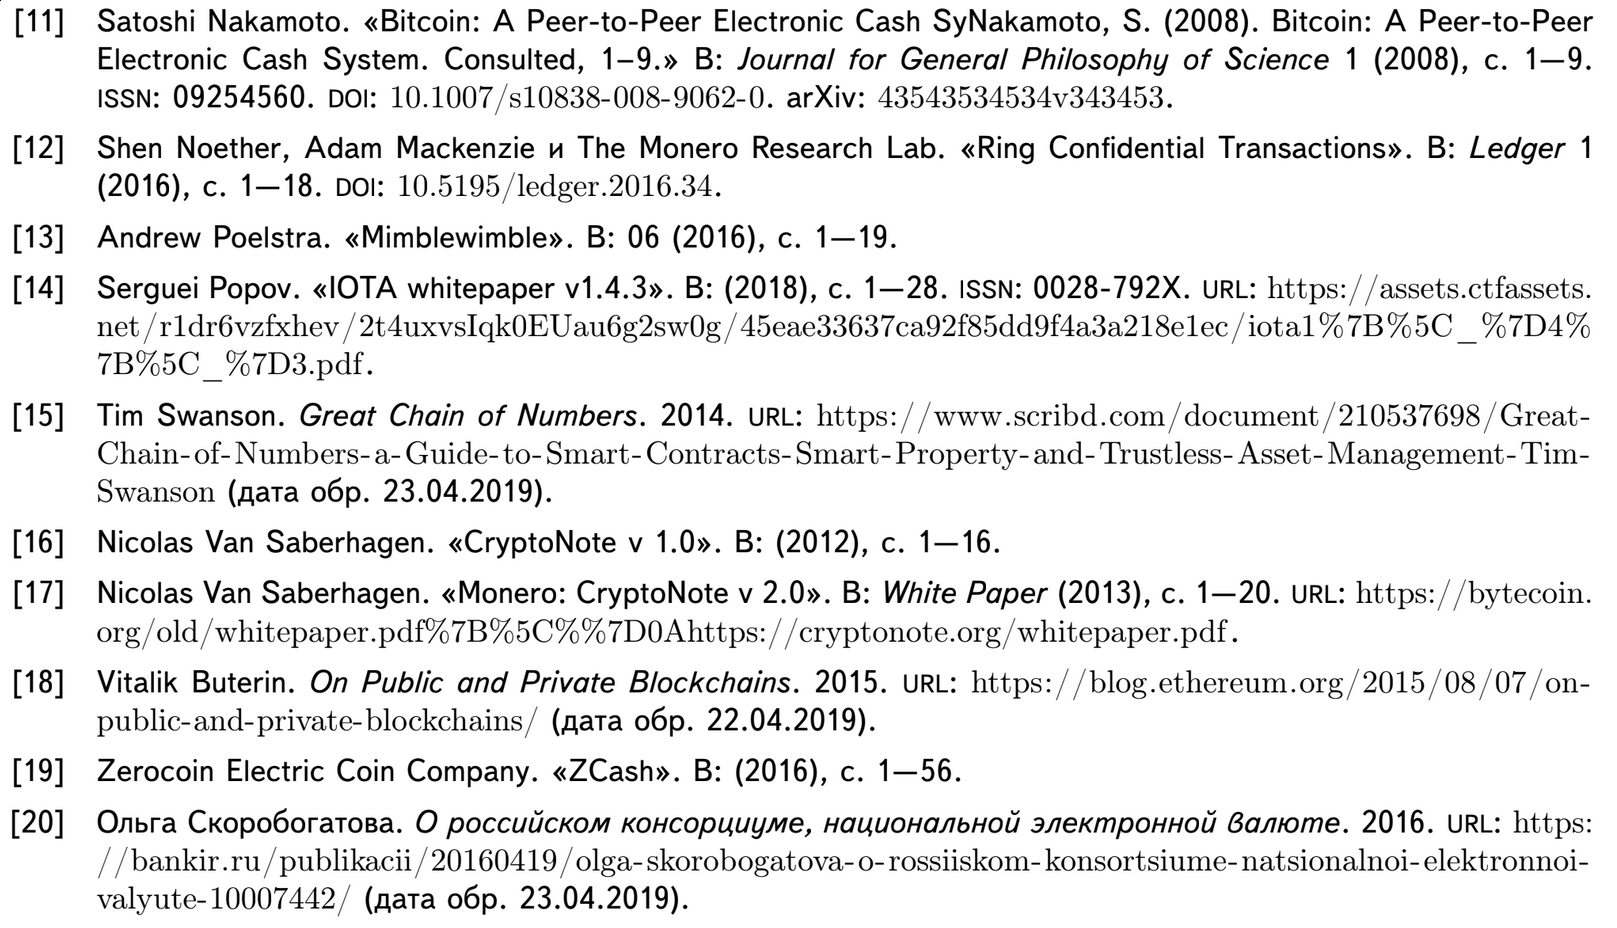
\includegraphics[width=\columnwidth]{lit2.png}
    \end{figure}
\end{frame}

\begin{frame}[c]
\begin{center}
\frametitle{\LARGE Спасибо за внимание!}

{\LARGE \inserttitle}

\bigskip

{\insertauthor}

\bigskip\bigskip

{\insertinstitute}

\bigskip\bigskip

{\large \insertdate}
\end{center}
\end{frame}

\end{document}


% EOF

